\documentclass[twoside,9pt]{article}
\usepackage{times}
\usepackage{amssymb}
\usepackage{amsfonts}
\usepackage[fleqn]{amsmath}
\usepackage{bm}
\usepackage{url}
\usepackage[ruled]{algorithm2e}

\usepackage{listings}
\lstset{aboveskip=0.2em,
  breaklines=true,
  commentstyle={\color{red}},
  escapeinside={``},
  floatplacement=tbp,
  frame=topline,
  keywordstyle={\color{blue}\ttfamily},
  language=Java,
  numbers=left,
  numberstyle={\small},
  tabsize=2,
  xleftmargin=2em,
  xrightmargin=0em}

\usepackage[a4paper]{geometry}
\geometry{verbose,tmargin=25mm,bmargin=25mm,lmargin=14.5mm,rmargin=14.5mm}

\setcounter{secnumdepth}{2}
\setcounter{tocdepth}{2}

\usepackage{float}
\usepackage{booktabs}
\usepackage{graphicx}
\usepackage{setspace}
\usepackage{tikz}
\usetikzlibrary{shapes,arrows}

%\onehalfspacing
\usepackage[unicode=false,pdfusetitle,
 bookmarks=true,bookmarksnumbered=true,bookmarksopen=false,
 breaklinks=true,pdfborder={0 0 1},backref=slide,colorlinks=true]
 {hyperref}
%\hypersetup{unicode=false}

\renewcommand{\labelenumi}{\alph{enumi})}
\usepackage{ccaption}

\makeatletter
%\providecommand{\tabularnewline}{\\}

\makeatletter
\let\@afterindentfalse
\@afterindenttrue
\@afterindenttrue
\makeatother
\setlength{\parindent}{2em}

\usepackage{xeCJK}
\usepackage{xltxtra}
\usepackage{xunicode}

%========================================================
% Here please change the fonts to similar ones in your computer
%========================================================
\setmainfont{Times New Roman}
\setsansfont{Candara}
\setCJKmainfont[BoldFont=Adobe Heiti Std,ItalicFont=Adobe Kaiti Std]{Adobe Song Std}

\XeTeXlinebreaklocale "zh"
\XeTeXlinebreakskip = 0pt plus 1pt minus 0.1pt
\renewcommand
\arraystretch{1.5}
\renewcommand{\contentsname}{目录}
\renewcommand{\listfigurename}{插图目录}
\renewcommand{\listtablename}{表格目录}
\renewcommand{\refname}{参考文献}
\renewcommand{\abstractname}{摘要}
\renewcommand{\indexname}{索引}
\renewcommand{\tablename}{表格}
\renewcommand{\figurename}{图}
\makeatother

\usepackage{fancyhdr}
\pagestyle{fancy}
\fancyhead{}%clear all settings
\fancyfoot{}%clear all settings
\fancyhead[RO,LE]{\thepage}
\renewcommand{\headrulewidth}{0.7pt}

\renewcommand{\baselinestretch}{1.2}

\newcommand{\chtitle}[1]{~\par\vspace{6pt}{\fontsize{20pt}{\baselineskip}\bf\selectfont#1}\par\vspace{18pt}}
\newcommand{\chauthor}[1]{{\fontsize{14pt}{\baselineskip}\selectfont#1}\par\vspace{16pt}}
\newcommand{\chaffiliation}[1]{{\fontsize{10pt}{\baselineskip}\selectfont(南京大学 计算机科学与技术系, 南京 210046)}\par\vspace{16pt}}
\newcommand{\entitle}[1]{{\fontsize{16pt}{\baselineskip}\bf\selectfont#1}\par\vspace{12pt}}
\newcommand{\enauthor}[1]{{\fontsize{10pt}{\baselineskip}\selectfont#1}\par\vspace{12pt}}
\newcommand{\enaffiliation}[1]{{\fontsize{9pt}{\baselineskip}\selectfont(Department of Computer Science and Technology, Nanjing University, Nanjing 210046, China)}\par\vspace{28pt}}
\newcommand{\enabstract}[1]{{\fontsize{10pt}{\baselineskip}\selectfont{\bf Abstract:~}#1}\par\vspace{12pt}}
\newcommand{\enkeywords}[1]{{\fontsize{10pt}{\baselineskip}\selectfont{\bf Keywords:~}#1}\par\vspace{12pt}}

\renewcommand{\labelenumi}{\bfseries{\alph{enumi}.}}
\renewcommand{\labelenumii}{\bfseries{\arabic{enumii}.}}

\newcommand\abs[1]{\left\lvert #1 \right\rvert}
\newcommand\floor[1]{\left\lfloor #1 \right\rfloor}
\newcommand\ceil[1]{\left\lceil #1 \right\rceil}
\newcommand\yin[1]{\textit{#1}}
\newcommand\yang[1]{\textbf{#1}}

%=======================================================
% Document begins
%=======================================================
\begin{document}


\begin{flushleft}
	\noindent
	\chtitle{利用综合传感器进行活动识别}  %<== use your own words
	\chauthor{李健 (学号: 101220055)} %<== use your own words
	\chaffiliation
	\par\par
	\entitle{\large Activity Recognition using integrated sensors} %<== use your own words
	\enauthor{Jian Li} %<== use your own words
	\enaffiliation
	
	\enabstract{
	The latest generation of smart mobile devices incorporates many diverse and powerful sensors.
	These sensors include GPS sensors, temperature sensors, audio sensors (i.e. microphones), light sensors, vision sensors (i.e. cameras), acceleration sensors (i.e. accelerometers), rotation sensors (i.e. gyroscopes) and direction sensors (i.e. magnetometers).
	The availablility of these sensors in mobile devices creates exciting new application in data mining.
	In this paper we describe and evaluate a system that use various phone-based sensors to perform \yin{activity recognition}, a task which involves identifying the physical activity a user is performing.
	To implement our system we collected labeled sensors data from users as they performed 24 daily activities, and then aggregated this time series data into examples that summarize the user activity over several second intervals.
	We then used the resulting training data to induce a predictive model for activity recognition separately for each activity.
	Finally, we combine all the predicted results from the models of different activity and give the final recognition result.
	According to the online contest result, Sum of F1 is 10.3766 as well as the best single class F1 is 0.9938 (the worst single class F1 is 0.8577) which performs excellent for some situations.  
	}
	\enkeywords{data mining; activity recognition; sensors; data analysis; time series}
	
	\textbf{摘~~要:~~}\emph{
	时下流行的智能移动设备都具有多样强大的传感器。
	这些传感器包括GPS传感器,温度传感器,声音传感器(麦克风),光传感器,视觉传感器(摄像头),加速度传感器(加速计),旋转传感器(陀螺仪),方向传感器(磁力计)。
	具备这些传感器的移动设备使得数据挖掘有了更多的新应用。
	在这篇文章中,我们描述并评估一个基于多种手机传感器的活动识别的系统,这个系统可以识别用户在物理世界中的活动。
	为了实现我们的系统,我们收集了24种用户日常活动的具有label的传感器数据,然后对这些时间序列的数据进行处理,并在几秒的单位时间内对用户活动进行刻画。接下来,我们利用所有产生的训练数据,对每一个独立的活动建立预测其模型。最终,我们合并所有活动模型预测的结果,并给出最终的预测结果。
	根据在线竞赛的结果,F1的和为10.3766,同时最好的单类F1为0.9938(最差的单类F1为0.8577),这一结果说明在某些情形下,系统预测结果非常出色。
	}
	\textbf{关键词:~~}  数据挖掘;活动识别;传感器;数据分析;时间序列\\
	\textbf{中图法分类号:~~TP301   文献标识码: A}
\end{flushleft}

\vspace{12pt}
%\thispagestyle{empty}

%========================
% Body of the report
%========================


\section{引言}

%a) 叙述你的想法(要做什么、有何意义)。
%b) 详细描述出其中的数据挖掘问题。
%c) 大体介绍所使用的解决方案(基于如何的想法、有怎样的关键步骤),以及实验获得的效果

移动设备,例如智能手机、平板电脑以及音乐播放器,时下都配备了多样强大的传感器。这些传感器包括GPS传感器,温度传感器,声音传感器(麦克风),光传感器,视觉传感器(摄像头),加速度传感器(加速计),旋转传感器(陀螺仪),方向传感器(磁力计)。由于这些移动设备体系小方便携带,并且具备强大的计算能力,可以时时通过网络进行数据交互,这为数据挖掘的研究和应用提供了新的平台。在这篇文章中,我们将介绍一种利用加速计、陀螺仪以及磁力计来进行用户活动识别的方法。这一方法可以在移动设备上得到广泛的应用。\cite{CC}

很明显,这是一个数据挖掘领域中的分类问题。首先,我们通过一些已知活动label的传感器训练数据来建立预测模型,并利用该预测模型来对未知活动label的传感器数据进行预测分类,即实现活动识别。

在本文中,介绍了该问题的一种有效的解决方案。首先,我们需要收集用户日常活动行为的传感器数据,记录该活动信息并给予一个活动编号;之后,我们将所有这些收集的数据进行预处理,将其分解成不同活动,压缩数据并从中提取特征值;利用这些处理过的数据,为不同的活动分别建立预测模型,调节模型相应的参数,使其具有较高的预测准确度;这一模型的作用,是根据未知活动类别的传感器数据,来判断其是否符合该模型,做出相应判断;当所有活动模型都对未知数据做出判断后,最终由仲裁系统来最终判定这一数据所应该对应的活动。

实验结果如下:
\begin{tabular}{ c | c | c }
	$\sum F_1$ & Best single class $F_1$ & Worst single class $F_1$ \\\hline
	10.3766 & 0.9938 & 0.8577
\end{tabular}

这一结果证明,该方法有着良好的实际表现。

本文后续部分组织如下: 第2节回顾相关工作,第3节详细陈述使用的数据挖掘方法,第4节报告实验结果,第5节对讨论本文的方法并总结全文。

\section{相关工作}

%[对他人做过的类似的工作进行回顾(他人解决的问题和你的问题有何相似或不同、采取的什么想法、使用了什么方案)]
在活动识别这个领域前人已经做过很多研究工作\cite{DD}。Bao \& Intille\cite{AA} 设计了一个活动识别系统利用5个放置在用户身体不同位置上的加速计来识别20种不同的活动。类似的,更多的研究关注于怎么利用多种加速计来识别用户活动范围。更多的工作关注于基于加速计的活动识别系统的应用。值得一提的是,Jennifer, Gary \& Samuel\cite{CC}的工作与之前的工作有所不同,他们使用的是时下随处可见的真实的移动设备,而不是专业的研究设备;此外,他们的设备只需要用户放置在用户的口袋中,而不是穿戴在身体上,不需要增加用户的而外工作。

我们的工作有如下几点贡献。首先,我们使用的传感器种类更加多样,这其中包括之前没有使用过的温度传感器、磁力计以及陀螺仪,这无疑使得我们在活动识别中拥有更多的可以利用的资源;此外,我们的工作中更注重的是从数据中提取特征,并归约为经典的分类问题,可以使用传统的分类算法;最后,我们的系统在数据处理、特征提取、训练以及预测过程中,极为高效,使得我们的系统可以处理实时请求并动态反馈我们的系统。

\section{本文的方法}

%[介绍本文使用的方法的思想]
%[展开详细介绍使用的方法,使得读者可以自行实现相同的方法。本节中可以划分小节。]

%Figure Diagram
\tikzstyle{A} = [draw, thin, fill=blue!20]
\tikzstyle{B} = [ellipse, draw, thin, fill=green!20, minimum height=2.5em]

\begin{tikzpicture}[node distance = 3.8cm, auto, >=latex', thick]
	\node [A] (compress) {Compression};
	\node [B, below of=compress] (data) {Sensors Data};
	\node [A, right of=compress] (fe) {Feature Extration};
	\node [A, right of=fe] (classification) {Classification};
	\node [A, right of=classification,node distance = 4.2cm] (model) {Model};
	\node [B, below of=model] (result) {Result};
	\node [A, left of=result] (arbiter) {Arbiter};
	\node [B, left of=arbiter] (label) {Label};
	\node [A, node distance = 1.9cm, below of=compress] (split) {Split};

	\path[->] (compress) edge (fe);
	\path[->, dashed] (fe) edge (classification);
	\path[->, dashed] (classification) edge node[auto,midway] {Training} (model);
	\path[->] (model) edge (result);
	\path[->] (fe) edge [bend left] (model);
	\path[->] (model) edge node[auto,midway] {Prediction} (result);
	\path[->,dashed] (result) edge node[auto,midway,above] {Recovery} (arbiter);
	\path[->,dashed] (result) edge [bend left] (arbiter);
	\path[->,dashed] (result) edge [bend right] (arbiter);
	\path[->] (arbiter) edge (label);
	\path[->] (data) edge (split);
	\path[->,dashed] (split) edge (compress);
	\path[->,dashed] (split) edge [bend left] (compress);
	\path[->,dashed] (split) edge [bend right] (compress);

\end{tikzpicture}

\subsection{数据收集}

我们的数据来源于穿戴在用户身上的综合传感器,其中包括
\begin{itemize}
	\item	$1 \times$心跳传感器(未使用)
	\item	$3 \times$综合传感器
		\begin{itemize}
			\item	$1 \times$ 温度传感器
			\item	$1 \times$ Type I  3D加速计
			\item	$1 \times$ Type II 3D加速计
			\item	$1 \times$ 3D陀螺仪
			\item	$1 \times$ 3D磁力计
		\end{itemize}
\end{itemize}

所以,数据总共由41 Features组成。Label的编号为0$\sim$24,其中0表示没有活动;实际上,所有给出的训练数据中仅仅出现了1, 2, 3, 4, 5, 6, 7, 12, 13, 16,17, 24这12个活动,对于其他的活动,没有相应的数据,我们也不能对其描述。

\subsection{数据处理}

\begin{figure}[H]
	\centering
	\label{FB}
	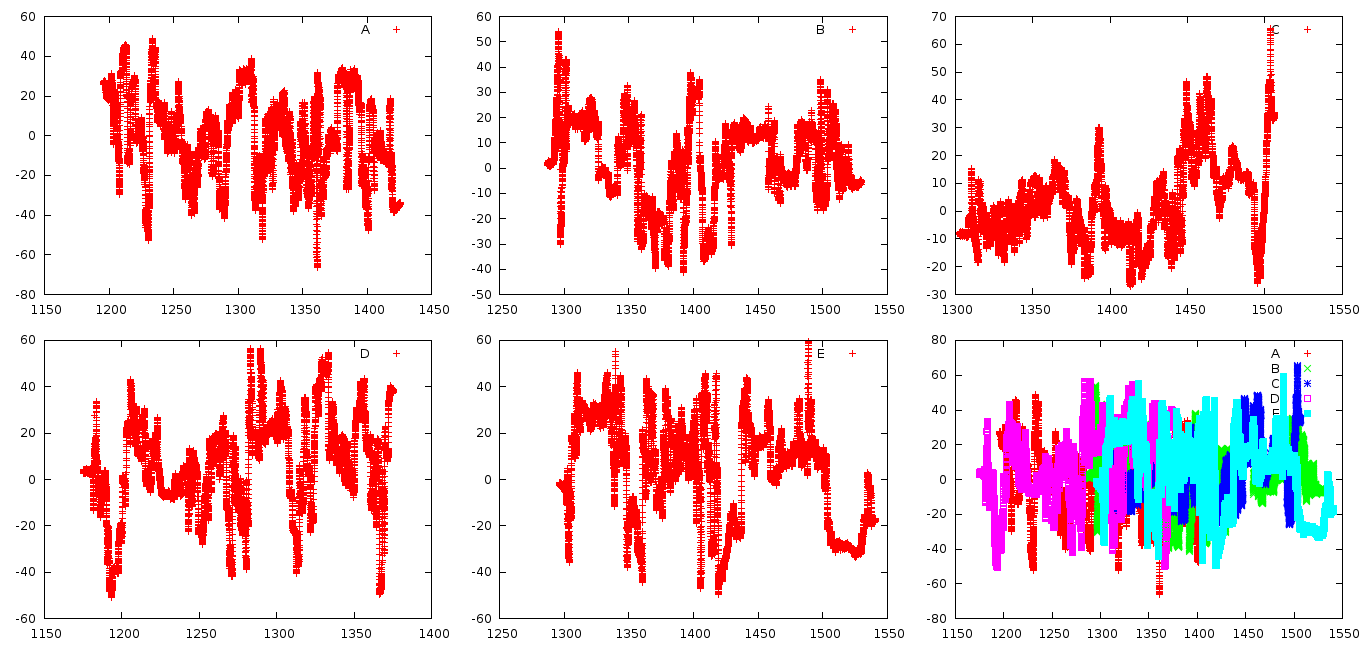
\includegraphics[width=1\textwidth]{B.png}
	\bicaption{图\ref{FB}}{不同数据集中同一活动离散时间序列数据}{Figure}{Discrete time-series data of the same activity in different data set}
\end{figure}

\subsubsection{分离}
原始传感器数据包含了多种活动类型的数据,由于我们随后是要对不同的活动类型分别进行刻画建模,所以首先我们需要将所有数据根据label来进行分离(splitting),将所有属于该活动的数据label映射为1,不属于的映射为-1。这样原始的Multi-class classification问题,就归约为Two-class classification问题。

\subsubsection{压缩}
原始的传感器数据中,由于心跳传感器和综合传感器的采样频率不一至,所以我们决定放弃使用心跳传感器。同时,传感器数据采样过于频繁,导致数据量极为庞大,其中还包括许多丢失的数据,所以第二步对数据的处理就是压缩(compression)。我们使用的方法就是对连续的$\alpha$次数据进行平均,如果其中包含丢失的值,则在剩下已知的数据中求平均;此处,我们引入第一个参数$\alpha$。对原始数据进行平均,有三个优点:
\begin{enumerate}
	\item	压缩原始的数据,使得数据规模减小$\alpha$倍,在后面训练预测过程中,有着更好的性能
	\item	通过观察原始数据,在一定时间尺度下,我们可以认为数据是连续的,那么对于丢失的数据,可以通过其时间点附近的数据来还原,即压缩过程中完成了未知数据还原操作
	\item	压缩使得数据更加平滑(smooth),这就间接的消除了一些异常数据点所造成的影响
\end{enumerate}

\subsection{数据变换 \& 特征提取}

所有的数据都是基于连续时间序列(time-series)的,对于通常的分类算法,不能直接处理原始时间序列的数据\cite{BB}。所以我们需要对一段时间内的数据进行变换或是特征提取,使得新的费时间序列数据可以有效的刻画原始的序列数据。在此,我们引入第二个参数$\beta$,表示将$\beta$个处理后的数据放入一个时间段中进行刻画,即数据再次压缩了$\beta$倍。

\begin{figure}[H]
	\centering
	\label{FA}
	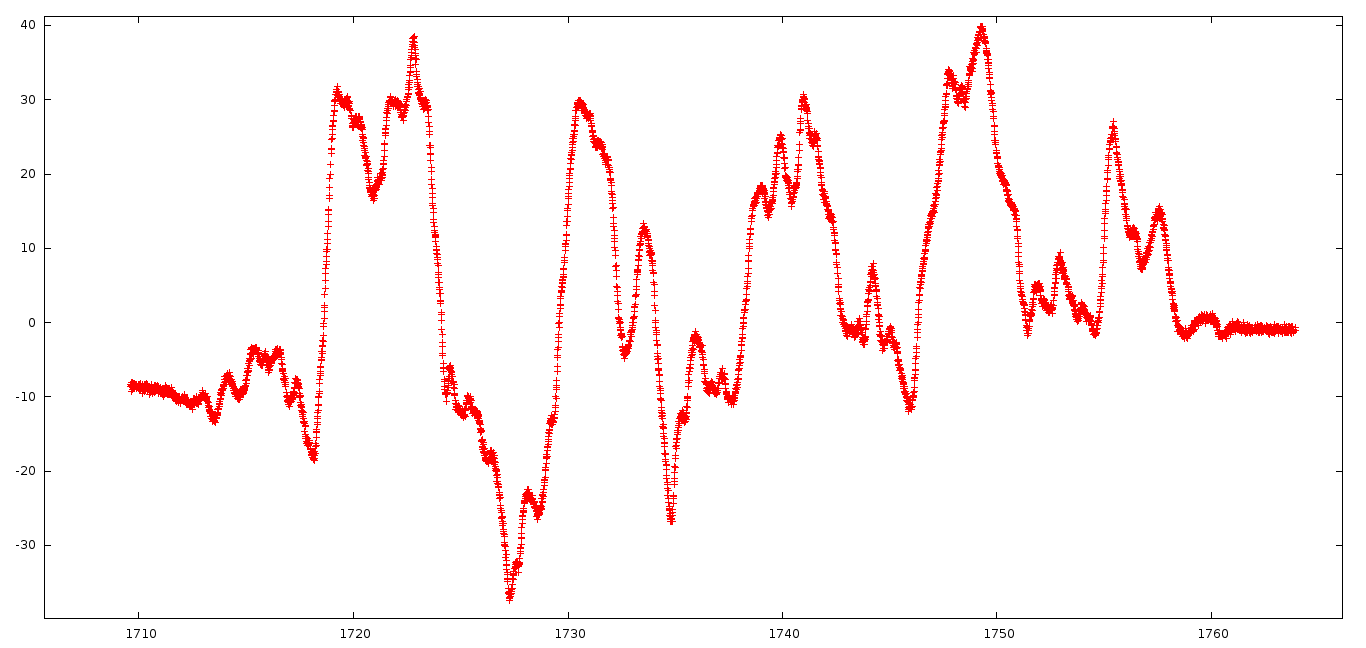
\includegraphics[width=1\textwidth]{A.png}
	\bicaption{图\ref{FA}}{离散时间序列数据}{Figure}{Discrete time-series data}
\end{figure}


接下来,我们需要解决的问题,就是对一段内的数据生成新的非时间序列的features。由于数据具有高度的时间连续性,问题可以进一步抽象为如何准确刻画一个$x$-$t$函数。在此我们使用了如下方法\cite{CC}\cite{DD}:

\begin{itemize}
	\item	Average\\
			所有数据点的平均值
	\item	Standard Deviation\\
			所有数据点的标准差	
	\item	Maximum-Minimum Difference\\
			最大点数据与最小数据点的差
	\item	Head-Tail Difference\\
			首尾数据点的差
	\item	Average Absolute Difference\\
			所有数据点至平均值的距离的绝对值的平均值	
	\item	Time between Peaks\\
			数据中峰值点之间的平均时间,该feature可以一定程度上刻画数据的周期性
	\item	Binned Distribution\\
			数据点在不同范围内的分布
	\item	Discrete Wavelet Transform: Haar
			离散Haar小波变换
\end{itemize}

以下我们重点介绍后三种features。

\subsubsection{Time between Peaks}
为了计算峰值点之间的平均时间,我们需要解决连续时间序列数据中峰值检测问题。这一问题具有诸多heuristic的方法,在此我们使用一简单有效的算法\cite{GG}

\begin{figure}[H]
	\centering
	\label{FC}
	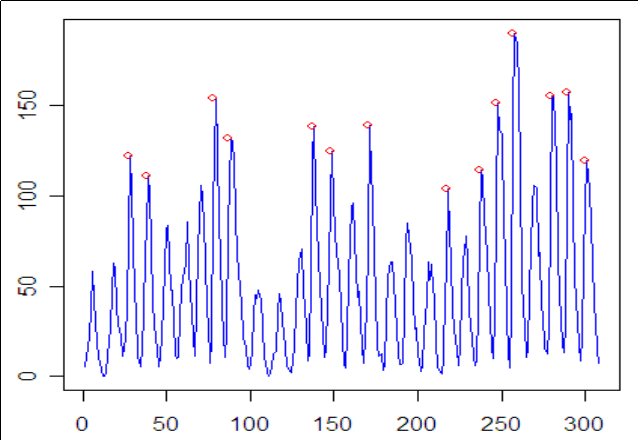
\includegraphics[width=0.6\textwidth]{C.png}
	\bicaption{图\ref{FC}}{峰值检测}{Figure}{Peaks Detection}
\end{figure}

\begin{algorithm}[H]
	\caption{Peak Detection Algorithm that uses Peak Function F}
	\DontPrintSemicolon
	\SetKwInOut{Input}{Input}
	\SetKwInOut{Output}{Output}
	\SetKw{And}{and}
	\Input{Time-series of $N$ points: $X = \{x_1, x_2, \cdots, x_N\}$, $N$ \\  Window size around the peak: $K$ \\ Threshold: $H$}
	\Output{Set of peaks detected in $X$: $S$}
	\BlankLine
	\Begin{
		$S = \emptyset$\;
		\For{$i = 1$ \KwTo $N$}
		{
			$A[i] = F(X, i, K)$\;
		}
		Compute the mean $avg$ and standard deviati n $var$ of all values in array $A$\;
		\For{$i = 1$ \KwTo $N$}
		{
			\If{$A[i] > 0$ \And $(A[i] - avg) > H \cdot var$}
			{
				$S = S \cup \{x_i\}$\;
			}
		}
		\For{every adjacent pair of peaks $x_i$ and $x_j$ in $S$}
		{
			\If{$|j - i| \leq K$}
			{
				Remove the smaller value of $\{x_i, x_j\}$ from $S$\;
			}
		}

	}
\end{algorithm}

在这里,我们使用的Peak Function为
\begin{equation} \notag
	F(X, i, K) = x_i - \frac{\sum_{j \in [i - K, i + K] \backslash \{i\}} x_j}{2k}
\end{equation}
这一函数可以识别非常明显的峰值,如果希望识别所有可能的峰值,建议使用Entropy作为Peak Function。


\subsubsection{Binned Distribution}

首先,我们计算所有数据点的最大最小值之差,然后将这一范围分为10个等范围的bins,然后统计所有数据点落在这些bins的数量。

\subsubsection{Discrete Wavelet Transform: Haar}

在此,我们使用经典的1D Haar Wavelet Transform的算法,在此不做赘述。经过变换后,我们选择绝对值最大的5个元素作为Features。\cite{FF}

\subsubsection{刻画}

综合上述,我们将原来的1个时间序列的feature扩展为新的多维features,\yang{合理使用}这些features,可以有效的刻画原来基于时间序列的feature。


\subsection{训练预测}

对于提取后的特征,我们就可以使用经典的Two-Class Classification模型算法来进行学习训练,例如基于Decision Tree的C5.0算法,基于Neural Network的BP算法或是Support Vector Machine。建立好相应的模型后,就可以对做了相同处理的未知label的数据进行预测。

我们使用的方法是SVM with RBF kernel。\cite{EE}

\subsection{恢复原始数据}
第一、二步,我们将原始数据压缩,并进行特征提取,所以最后我们需要将预测后的结果进行扩展,恢复原始数据所对应的label。

\subsection{仲裁预测结果}
由于我们将不同活动分别建立不同的模型,所以最终我们拥有所有模型给出的预测结果,我们需要根据这些结果,最终决定该活动的类型。我们设计了一个仲裁系统\yang{Arbiter}来实现这一功能,其主要功能为

\begin{enumerate}
	\item	收集所有模型的预测结果
	\item	如果对该数据只有一个模型预测结果为positive (Confirmed),那么就分配该模型对应的label
	\item	如果没有任何一个模型预测的结果为positive (Unknown),那么就认为没有活动,分配0
	\item	如果有两个以上的模型预测的结果为positive (Confused),这个时候就需要根据不同模型的可靠度以及其他因素来综合判定,这一过程具体化为计算不同模型的分数,最终分配得分最高的模型对应的label
\end{enumerate}

由于在研究过程中数据有限,如果能将预测结果时时反馈给该系统,可以进一步设计时时动态仲裁系统。

\section{实验}

\subsection{实验设置}
%[详细交代实验的设置,使得读者可以重复该实验]
本实验使用的是\url{http://cs.nju.edu.cn/yuy/course_dm13_a2.ashx}所提供的训练及预测数据。其中提供了12种有效的活动传感器数据。

不同的活动其数据形态亦不同,所以我们需要不同的参数及特征来更好的刻画这些活动。所有参数如表格\ref{C1}

\begin{table}[h]
	\bicaption{表}{参数}{Table}{Parameters}
	\label{C1}
	\centering
	\begin{tabular}{cccccccc}
		\toprule
		Activity & $\alpha$ & $\beta$ & Training Data & Temperature & Haar & Time between Peaks & Binned Distribution\tabularnewline
		\midrule
		1 & 40 & 20 & ABCDE & + & - & + & +\tabularnewline
		2 & 50 & 20 & DE & - & + & - & -\tabularnewline
		3 & 10 & 100 & BCDE & - & + & - & -\tabularnewline
		4 & 50 & 20 & ABCDE & - & - & - & +\tabularnewline
		5 & 50 & 50 & BDE & - & - & + & +\tabularnewline
		6 & 50 & 20 & ABCDE & - & - & - & +\tabularnewline
		7 & 50 & 20 & ABCDE & - & - & - & +\tabularnewline
		12 & 50 & 20 & ABDE & + & + & - & -\tabularnewline
		13 & 50 & 50 & BDE & - & - & - & +($|Bins|=5$)\tabularnewline
		16 & 50 & 20 & ABCDE & + & + & - & -\tabularnewline
		17 & 50 & 50 & ABCDE & - & + & - & -\tabularnewline
		24 & 50 & 20 & ABCDE & + & - & + & +\tabularnewline
		\bottomrule
	\end{tabular}
\end{table}

\subsection{实验结果}
对于预测数据集X,我们的实验结果如表格\ref{CC}

\begin{table}[h]
	\bicaption{表}{实验结果}{Table}{Experiment Result}
	\label{CC}
	\centering
	\resizebox{1\textwidth}{!}{
	\begin{tabular}{cccccccccccccccc}
		\toprule
		Activity & 1 & 2 & 3 & 4 & 5 & 6 & 7 & 12 & 13 & 16 & 17 & 24 & Sum & Best & Worst\tabularnewline
		\midrule
		$F_1$ & 0.9938 & 0.9884 & 0.9763 & 0.9451 & 0.9872 & 0.9372 & 0.9690 & 0.8577 & 0.8681 & 0.8819 & 0.9718 & N/A & 10.3766 & 0.9938 & 0.8577\tabularnewline
		\bottomrule
	\end{tabular}
}
\end{table}



%[如果有多种实验,可以组织在不同的小节中]
%[描述实验获得的客观结果,应当提供适当的图表]
%[讨论实验结果的含义]

\section{讨论与结束语}

对于本文提出的方法,其中仍存在着诸多有待提高之处:
\begin{enumerate}
	\item	对于每一类活动,训练的数据无论从准确程度还是规模来说,都不能很好支持我们的模型
	\item	实验所提供的参数,均从预测数据集X的反馈得来,可以说,我们的参数并不是最优的
	\item	通过实验的结果,我们发现我们的features对于12、13和16这三类活动刻画的并不充分
	\item	如果能有时时反馈的应用,\yang{Arbiter}系统可以设计的更为复杂,效果也会更好
	\item	对于每一类活动,我们现在仅仅是用一个模型来代表,我们可以使用Ensemble learning的方法,进一步提高准确度
	\item	可以继续尝试提取更多特征,及更有效的数据处理方法
\end{enumerate}

%[讨论本文的方法有何不足和有待提高之处,可能的解决方案有哪些]
%[对本文工作进行总结]

本文介绍了一种利用综合传感器来进行活动识别的方法,该方法使得我们可以使用经典的Two-Class Classification算法来解决该问题。
在数据处理过程中,我们将不同活动类型的数据分离并压缩,之后通过不同的方法来提取时间序列数据的特征,例如Discrete Wavelet Transform、Binned Distribution、Time between Peaks等。
提取特征后的数据,就可以使用经典Classification来训练以及预测。最终由仲裁系统来判定,该活动的label。通过实验证明,我们的方法是有效。


\appendix

\bibliographystyle{plain}
\phantomsection\addcontentsline{toc}{section}{\refname}\nocite{*}

\bibliography{references_db}

\end{document}



%%插入三线表示例%%
%\begin{table}[h]
%	\bicaption{表}{宏指令}{Table}{Macro Instructions}
%	\centering
%	\begin{tabular}{ccccc}
%		\toprule
%		Acronym & Macro-Instructions & Value & Symbol & Event symbol\tabularnewline
%		\midrule
%		NSI & NET\_SLICE\_INIT() & 87 & a & $\alpha$\tabularnewline
%		NST & NET\_SLICE\_STOP() & 154 & b & $\delta$\tabularnewline
%		NSE & NET\_SLICE\_EXIT() & 904 (1.4\%) & c & $\gamma$\tabularnewline
%		\bottomrule
%	\end{tabular}
%\end{table}

